
\documentclass{article}
\usepackage[a4paper]{geometry}
\usepackage{color}              % Controle das cores
\usepackage[utf8]{inputenc}
\usepackage[T1]{fontenc}
\usepackage[portuguese]{babel}
\usepackage{amsmath} % Permite diagramação matemática avançada
\usepackage{relsize}
\PassOptionsToPackage{hyphens}{url}\usepackage{hyperref} % Permite adicionar url's clicáveis
\usepackage{amssymb}
\usepackage{authblk}
\usepackage{tikz}
\usepackage{subfig}
\usepackage{float}
\usepackage{xcolor,colortbl}



\usetikzlibrary{matrix}

\DeclareMathOperator{\BigO}{O}

% Configura a exibição de urls
\hypersetup{
	colorlinks = true,
	urlcolor   = blue,
	linkcolor  = blue,
	citecolor  = black
}

\newenvironment{varalgorithm}[1]
{\algorithm\renewcommand{\thealgorithm}{#1}}
{\endalgorithm}



\title {\vspace{-3cm}EP 3 - Relatório}
\author{Felipe Constantino de Oliveira}
\affil{%
	MAC0417/5768 - Visão e Processamento de Imagens - IME-USP
}
\date{}
% ----
% Início do documento
% ----
\begin{document}
	
	\maketitle

	\section{Introdução}
	
	Este trabalho contém arquivos $.py$ e foi utilizada a seguinte configuração:
	\begin{itemize}
		\item Python 2.7
		\item OpenCV 3.4.1
		\item Numpy 1.14.3
		\item Matplotlib 2.1.2
		\item Scipy 1.1.0
	\end{itemize}
	
	\section{Problema 1}

	O primeiro desafio era utilizar os conceitos de Fourier para eliminar o ruído periódico na imagem do leopardo abaixo:
	
%	\begin{figure}[H]
%		\centering
%		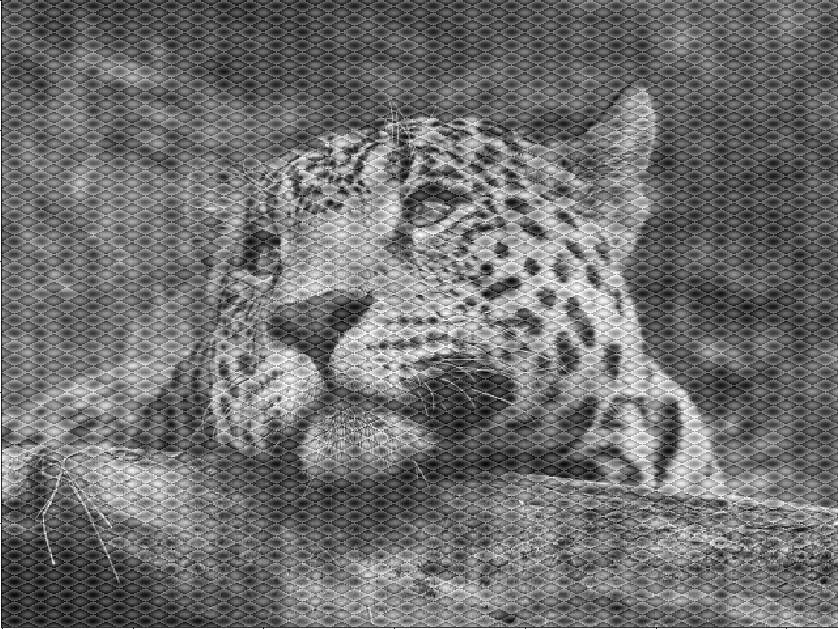
\includegraphics[scale=0.3]{images/1_original.png}
%		\caption{Imagem com Ruído periódico} 
%	\end{figure}
	
\end{document}



